%%%%%%%%%%%%%%%%%%%%%%%%%%%%%%%%%%%%%
%                                   %
% Compile with XeLaTeX and biber    %
%                                   %
% Questions or comments:            %
%                                   %
% joshua dot mcneill at uga dot edu %
%                                   %
%%%%%%%%%%%%%%%%%%%%%%%%%%%%%%%%%%%%%

\documentclass{beamer}
  % Read in standard preamble (cosmetic stuff)
  %%%%%%%%%%%%%%%%%%%%%%%%%%%%%%%%%%%%%%%%%%%%%%%%%%%%%%%%%%%%%%%%
% This is a standard preamble used in for all slide documents. %
% It basically contains cosmetic settings.                     %
%                                                              %
% Joshua McNeill                                               %
% joshua dot mcneill at uga dot edu                            %
%%%%%%%%%%%%%%%%%%%%%%%%%%%%%%%%%%%%%%%%%%%%%%%%%%%%%%%%%%%%%%%%

% Beamer settings
% \usetheme{Berkeley}
\usetheme{CambridgeUS}
% \usecolortheme{dove}
% \usecolortheme{rose}
\usecolortheme{seagull}
\usefonttheme{professionalfonts}
\usefonttheme{serif}
\setbeamertemplate{bibliography item}{}

% Packages and settings
\usepackage{fontspec}
  \setmainfont{Charis SIL}
\usepackage{hyperref}
  \hypersetup{colorlinks=true,
              allcolors=blue}
\usepackage{graphicx}
  \graphicspath{{../../figures/}}
\usepackage[normalem]{ulem}
\usepackage{enumerate}

% Document information
\author{M. McNeill}
\title[FREN2001]{Français 2001}
\institute{\url{joshua.mcneill@uga.edu}}
\date{}

%% Custom commands
% Lexical items
\newcommand{\lexi}[1]{\textit{#1}}
% Gloss
\newcommand{\gloss}[1]{`#1'}
\newcommand{\tinygloss}[1]{{\tiny`#1'}}
% Orthographic representations
\newcommand{\orth}[1]{$\langle$#1$\rangle$}
% Utterances (pragmatics)
\newcommand{\uttr}[1]{`#1'}
% Sentences (pragmatics)
\newcommand{\sent}[1]{\textit{#1}}
% Base dir for definitions
\newcommand{\defs}{../definitions}


  % Packages and settings

  % Document information
  \subtitle[Loisirs faits et \lexi{faire}]{Les loisirs que nous faisons et le verbe \lexi{faire}}

\begin{document}
  % Read in the standard intro slides (title page and table of contents)
  \begin{frame}
    \titlepage
    \tiny{Office: % Basically a variable for office hours location
Gilbert 121\\
          Office hours: % Basically a variable for office hours
 lundi, mercredi, vendredi 10:10--11:10
}
  \end{frame}

  \begin{frame}{}
    \begin{center}
      \Large Quiz
    \end{center}
  \end{frame}

  \begin{frame}{Révision du verbe \lexi{faire}}
    \begin{center}
      \begin{tabular}{l | l l | l l}
  \multicolumn{5}{c}{faire \gloss{to do}} \\
      & \multicolumn{2}{l |}{singulier} & \multicolumn{2}{l}{pluriel} \\
  \hline
  1re & je         & fais               & nous        & faisons \\
  2e  & tu         & fais               & vous        & faites \\
  \hline
  3e  & il (masc)  &                    & ils (masc)  & \\
      & elle (fem) & fait               & elles (fem) & font \\
      & on         &                    &             & \\
\end{tabular}

    \end{center}
  \end{frame}

  \begin{frame}{Les conjugaisons}
    \begin{enumerate}
      \item Est-ce que vous \underline{\uncover<2->{faites}} vos devoirs?
      \item Je ne \underline{\uncover<3->{fais}} pas le ménage le dimanche.
      \item Pourquoi est-ce que nous \underline{\uncover<4->{faisons}} du français?
      \item Jude et Judy \underline{\uncover<5->{font}} des randonnées en mai.
      \item Tu es paresseux! Tu ne \underline{\uncover<6->{fais}} pas grand-chose.
    \end{enumerate}
  \end{frame}

  \begin{frame}{Les activités des célébrités}
    \begin{columns}
      \column{0.5\textwidth}
        Qu'est-ce qu'ils font?
        \begin{enumerate}
          \item Michael Phelps
          \item[] \underline{\only<2->{Il fait de la natation.}}
          \item<3-> Leah Chase
          \item[] \underline{\only<4->{Elle fait la cuisine.}}
          \item<5-> Simone Biles
          \item[] \underline{\only<6->{Elle fait de la gym.}}
          \item<7-> Josephine Baker
          \item[] \underline{\only<8->{Elle fait de la danse.}}
          \item<9-> Bernard Hinault
          \item[] \underline{\only<10->{Il fait du vélo.}}
        \end{enumerate}
      \column{0.5\textwidth}
        \begin{minipage}[c][0.6\textheight]{\linewidth}
          \begin{center}
            \only<1-2>{
              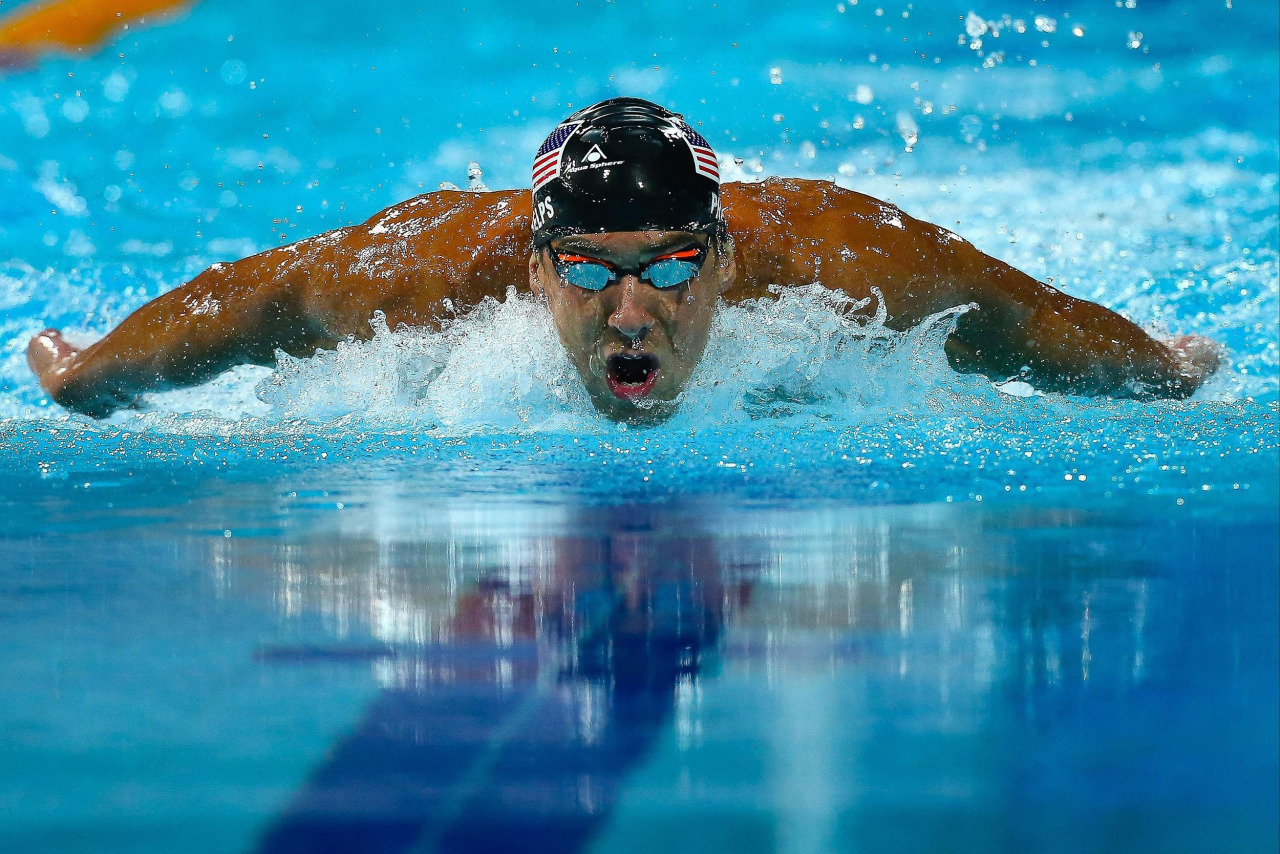
\includegraphics[scale=0.12]{michael_phelps.jpg}
            }
            \only<3-4>{
              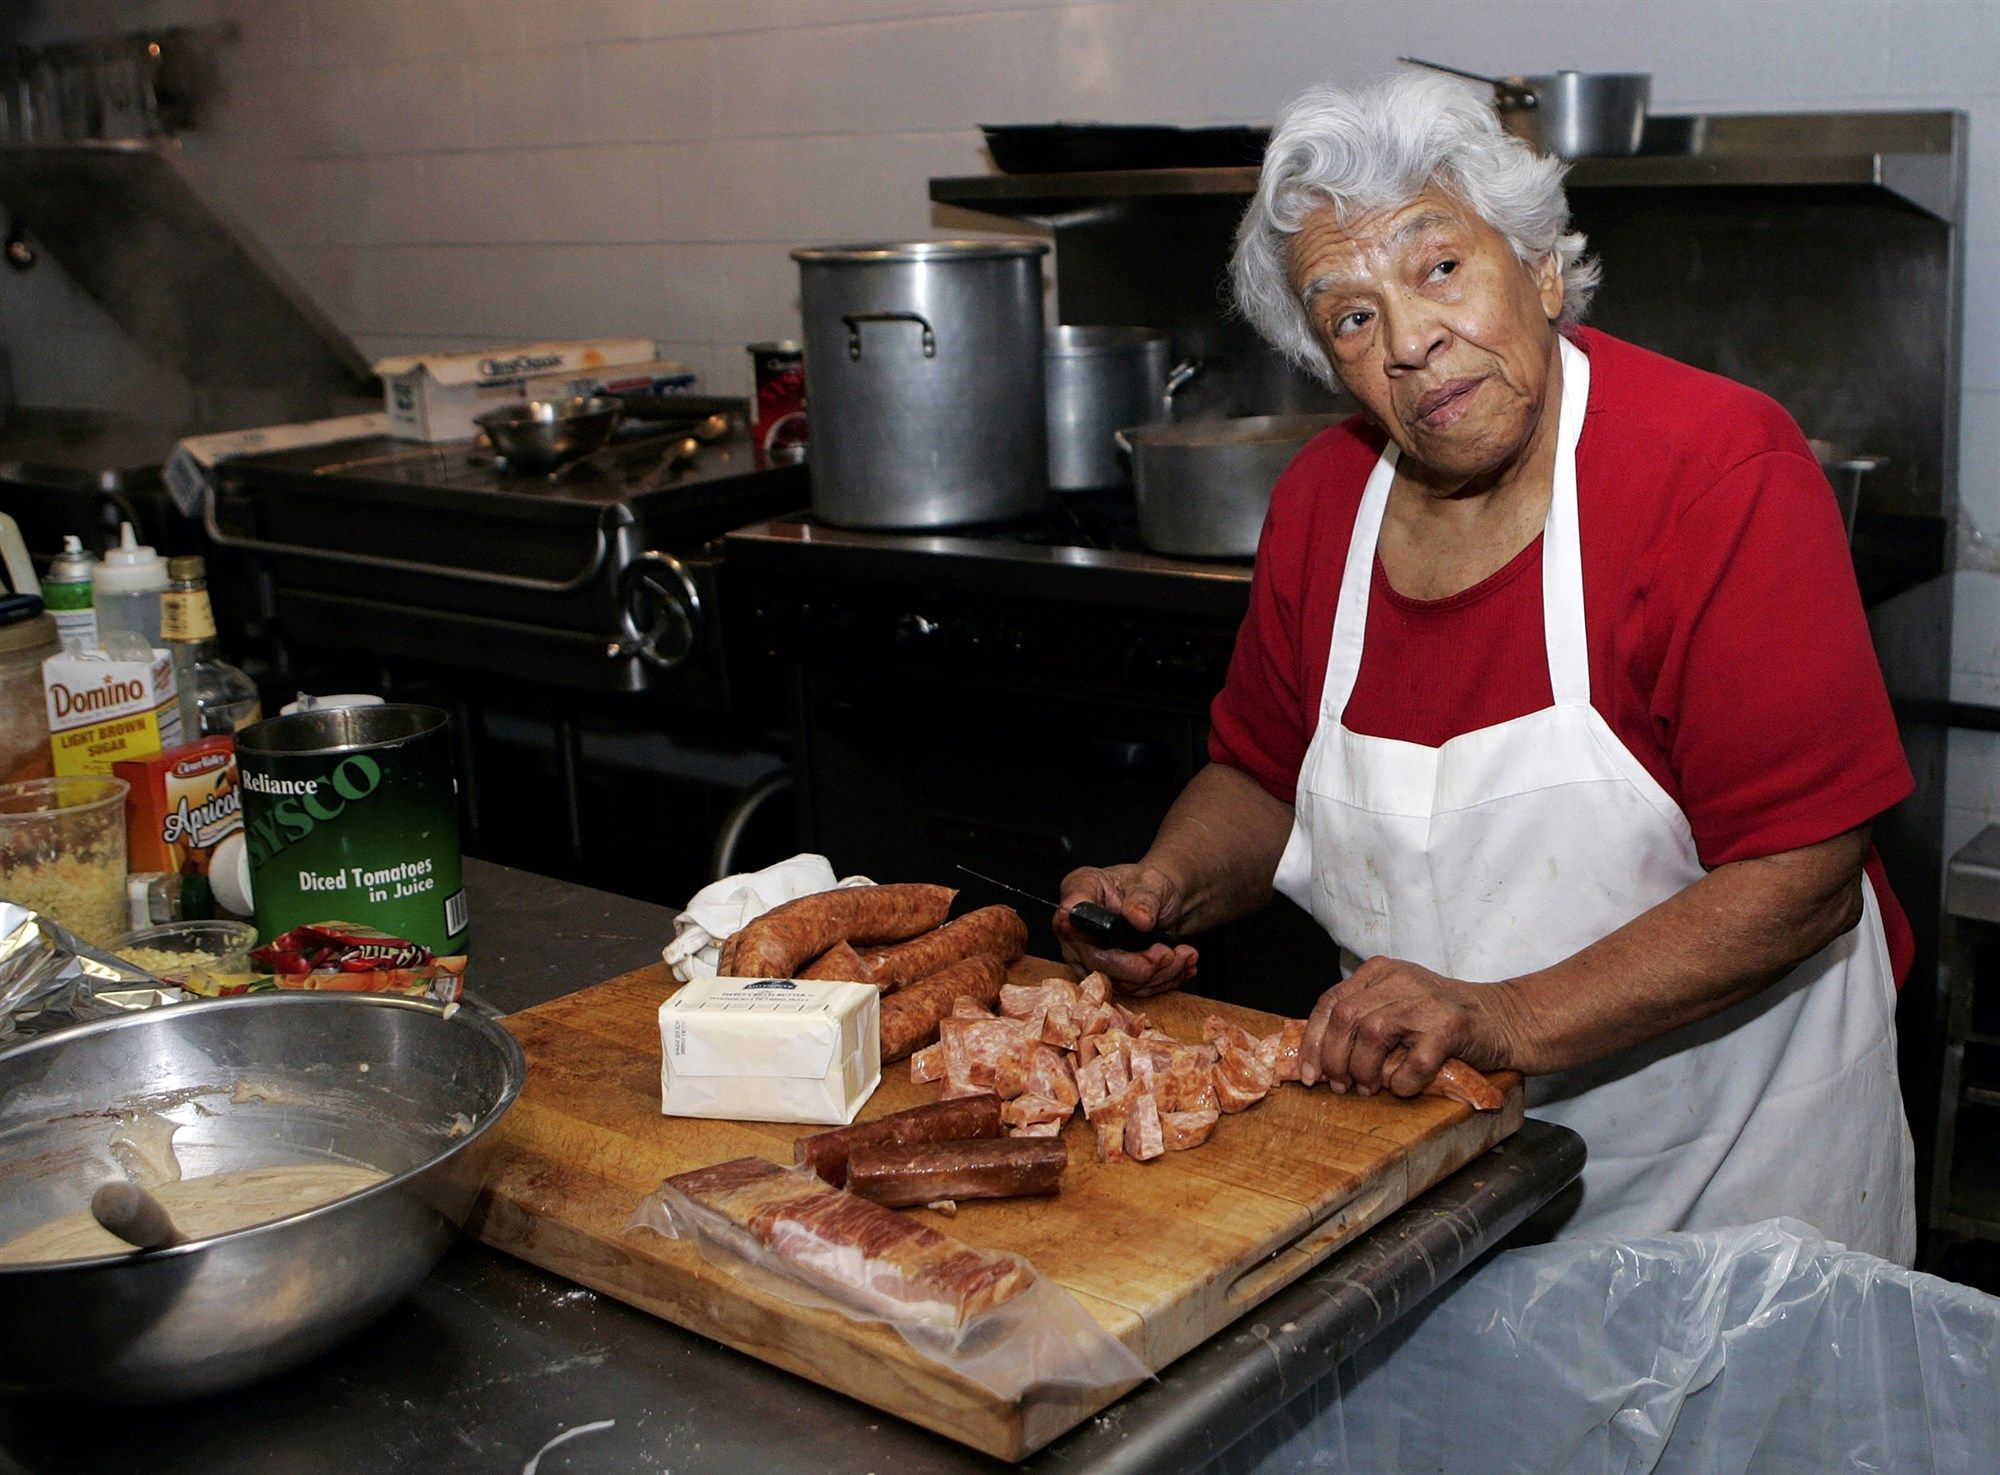
\includegraphics[scale=0.1]{leah_chase.jpg}
            }
            \only<5-6>{
              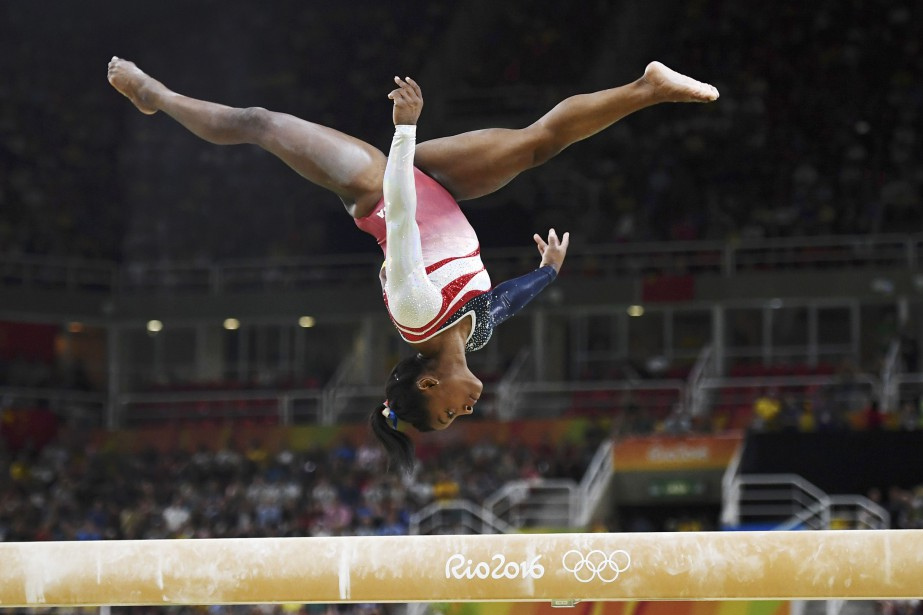
\includegraphics[scale=0.17]{simone_biles.jpg}
            }
            \only<7-8>{
              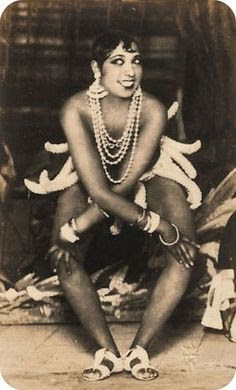
\includegraphics[scale=0.38]{josephine_baker.jpg}
            }
            \only<9-10>{
              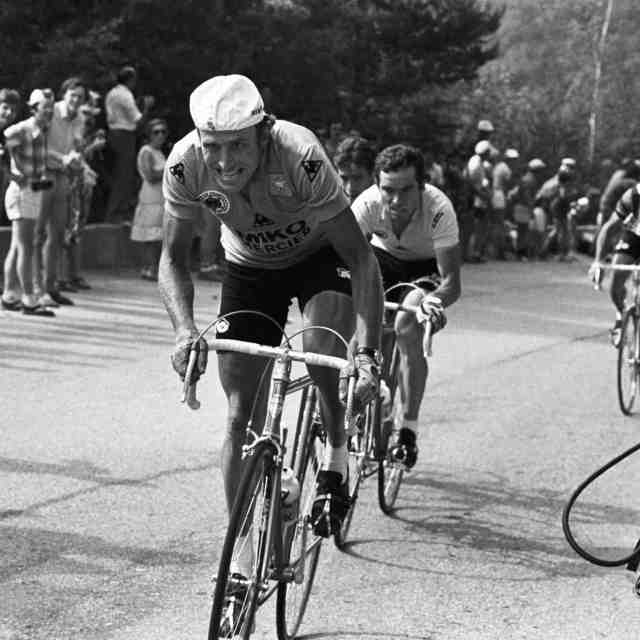
\includegraphics[scale=0.28]{bernard_hinault.jpg}
            }
          \end{center}
        \end{minipage}
    \end{columns}
  \end{frame}

  \begin{frame}{Un sondage}
    \begin{columns}
      \column{0.5\textwidth}
        \small
        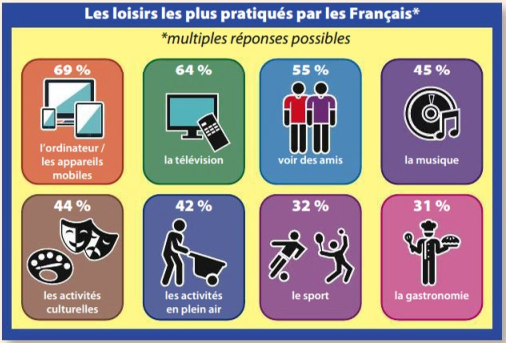
\includegraphics[scale=0.45]{loisirs_france.png} \\
        Les Français...
        \begin{itemize}
          \item travaillent 35 heures par semaine.
          \item prennent 5 semaines de vacances par année.
        \end{itemize}
      \column{0.5\textwidth}
        \small
        \begin{minipage}[t][0.8\textheight]{\linewidth}
        Comparons les Français avec la classe.
        En groupes de 5... \\
        \tinygloss{Let's compare the French with the class.
        In groups of 5...}
        \only<1>{
          \begin{enumerate}
            \item Demandez $\to$ \emph{Qui fait (du sport/de la musique/etc)?}
            \item[] \tinygloss{Ask $\to$ \emph{Who does (sports/music/etc)?}}
            \item Comptez les personnes
            \item[] \tinygloss{Count the people}
            \item Écrivez les résultats
            \item[] \tinygloss{Write the results}
          \end{enumerate}
        }
        \only<2>{
          \begin{enumerate}
            \item Annoncez les résultats $\to$ \emph{3 étudiants font du sport dans notre groupe.}
            \item[] \tinygloss{Announce your results $\to$ \emph{3 students do sports in our group.}}
            \item Un/e volontaire écrit le nombres sur le tableau
            \item[] \tinygloss{One volunteer writes the numbers on the board}
            \item Nous faisons les calculs pour le pourcentage de la classe
            \item[] \tinygloss{We calculate the percentage of the class}
          \end{enumerate}
        }
        \end{minipage}
    \end{columns}
  \end{frame}

  \begin{frame}{}
    \begin{center}
      \Large Questions?
    \end{center}
  \end{frame}
\end{document}
